%last edited 21.07.2015
\documentclass[11pt,reqno]{amsart}
\usepackage{amsmath,epsfig,graphicx,color}
%\usepackage[english,ngerman]{babel}
%\usepackage[latin1]{inputenc}
\usepackage{ifthen}
\usepackage{dsfont}
\usepackage{shadethm}
\usepackage{framed}
%\usepackage{pstricks}
%\usepackage{graphics}
%\usepackage{tocbibind}
%\usepackage{showkeys}
%\usepackage{units}
\usepackage{subfigure}
\usepackage{amssymb,latexsym}
%\usepackage{amsfonts}
%\usepackage{makeidx,showidx}
%\usepackage[sc]{mathpazo}
%\linespread{1.05}

%\usepackage[backref=page]{hyperref}
\usepackage{hyperref}
\hypersetup{
%linktoc=page,
%bookmarks=true, % show bookmarks bar?
%unicode=false, % non-Latin characters in Acrobat? bookmarks
%pdftoolbar=true, % show Acrobat? toolbar?
%pdfmenubar=true, % show Acrobat? menu?
%pdffitwindow=true, % window fit to page when opened
%pdfstartview={FitH}, % fits the width of the page to the window
pdftitle={Paper}, % title
pdfauthor={Johannes Heiny}, % author
pdfsubject={Title}, % subject of the document
%pdfcreator={Creator}, % creator of the document
%pvdfproducer={Producer}, % producer of the document
pdfkeywords={multivariate regular variation} , % list of keywords
%pdfnewwindow=true, % links in new window
%colorlinks=true, % false: boxed links; true: colored links
%linkcolor=blue, % color of internal links
%citecolor=blue, % color of links to bibliography
%filecolor=blue, % color of file links
%urlcolor=blue, % color of external links
urlcolor=black, 
  menucolor=black, 
  citecolor=black, 
  anchorcolor=black, 
  filecolor=black, 
  linkcolor=black, 
  colorlinks=true,
}

\textwidth 6.50in
\topmargin -0.50in
\oddsidemargin 0in
\evensidemargin 0in
\textheight 9.00in
%\pagestyle{plain}

\newcommand{\E}{\mathbb{E}}
\renewcommand{\P}{\mathbb{P}}
\newcommand{\1}{\mathds{1}}
\newcommand{\R}{\mathbb{R}}
\newcommand{\N}{\mathbb{N}}
\newcommand{\C}{\mathbb{C}}
\newcommand{\Z}{\mathbb{Z}}
\newcommand{\Var}{\operatorname{Var}}
\newcommand{\Fo}{\bar{F}}
\renewcommand{\b}[1]{\boldsymbol{#1}}
\newcommand{\Rq}{\mkern 1.5mu\overline{\mkern-1.5mu\R\mkern-3.0mu}\mkern 1.5mu}
\newcommand{\Frechet}{Fr\'{e}chet }
\renewcommand{\Finv}{F^{\gets}}
\DeclareMathOperator{\e}{e}
\newcommand{\inv}[1]{#1^{\gets}}
\newcommand{\x}{\boldsymbol{x}}
\newcommand{\y}{\boldsymbol{y}}
\newcommand{\X}{\boldsymbol{X}}
\newcommand{\Y}{\boldsymbol{Y}}
\newcommand{\bfZ}{\boldsymbol{Z}}
\newcommand{\0}{\boldsymbol{0}}
\newcommand{\dint}{\,\mathrm{d}}
\newcommand{\mB}{\mathcal{B}}
\newcommand{\norm}[1]{\|#1\|}
\newcommand{\twonorm}[1]{\|#1\|_2}
\newcommand{\inftynorm}[1]{\|#1\|_\infty}
\newcommand{\vep}{\varepsilon}
\newcommand{\nto}{n \to \infty}
\newcommand{\xto}{x \to \infty}
\newcommand{\lhs}{left-hand side}
\newcommand{\rhs}{right-hand side}
\newcommand{\fidi}{finite-dimensional distribution}
\newcommand{\rv}{random variable}
\newcommand{\tr}{\operatorname{tr}}
\newcommand{\anp}{a_{np}^{-2}}
\newcommand{\Zbar}{\overline{Z}}
\newcommand{\M}{\text{max}}
%\renewcommand*{\backref}[1]{}
%\renewcommand*{\backrefalt}[4]{%
%    \ifcase #1 (Not cited.)%
%    \or        (Cited on page~#2.)%
%    \else      (Cited on pages~#2.)%
%    \fi}

%von Schmock
\newcommand{\4}{\mathchoice{\mskip1.5mu}{\mskip1.5mu}{}{}}
\newcommand{\5}{\mathchoice{\mskip-1.5mu}{\mskip-1.5mu}{}{}}
\newcommand{\2}{\penalty250\mskip\thickmuskip\mskip-\thinmuskip} % after comma

\newcommand{\levy}{L\'evy}
\newcommand{\slln}{strong law of large numbers}
\newcommand{\clt}{central limit theorem}
\newcommand{\sde}{stochastic differential equation}
\newcommand{\It}{It\^o}
\newcommand{\sta}{St\u aric\u a}
\newcommand{\ex}{{\rm e}\,}

\def\theequation{\thesection.\arabic{equation}}
\def\tag{\refstepcounter{equation}\leqno }
\def\neqno{\refstepcounter{equation}\leqno(\thesection.\arabic{equation})}

\newtheorem{lemma}{Lemma}[section]
\newtheorem{figur}[lemma]{Figure}
\newtheorem{theorem}[lemma]{Theorem}
\newtheorem{proposition}[lemma]{Proposition}
\newtheorem{definition}[lemma]{Definition}
\newtheorem{corollary}[lemma]{Corollary}
\newtheorem{example}[lemma]{Example}
\newtheorem{exercise}[lemma]{Exercise}
\newtheorem{remark}[lemma]{Remark}
\newtheorem{fig}[lemma]{Figure}
\newtheorem{tab}[lemma]{Table}
\newtheorem{conjecture}[lemma]{Conjecture}

\newcommand{\cid}{\stackrel{d}{\rightarrow}}
\newcommand{\cip}{\stackrel{\P}{\rightarrow}}

\newcommand{\var}{{\rm var}}
\newcommand{\med}{{\rm med}}
\newcommand{\cov}{{\rm cov}}
\newcommand{\corr}{{\rm corr}}
\newcommand{\as}{{\rm a.s.}}
\newcommand{\io}{{\rm i.o.}}
\newcommand{\Holder}{H\"older}

\newcommand{\cadlag}{c\`adl\`ag}

%--------------------------------------------------------------------------------------------
\begin{document}
\today
\bibliographystyle{plain}
\title[The sample covariance matrix of a heavy-tailed multivariate time series]{Recent advances in random matrix theory applied to heavy-tailed multivariate time series}

\begin{abstract}

\end{abstract}

\maketitle
\tableofcontents


%------------------------------------------------------------------------
\section{Introduction}\setcounter{equation}{0}

\subsection{Motivation: Lam + Yao, PCA, indices of upper/lower tails of S\&P
  components}
Figure \ref{fig:SP500_tail_indices} shows the estimated lower- and upper-tail indices of stocks
included in the S\&P 500 index.
\begin{figure}[htb!]
  \centering
  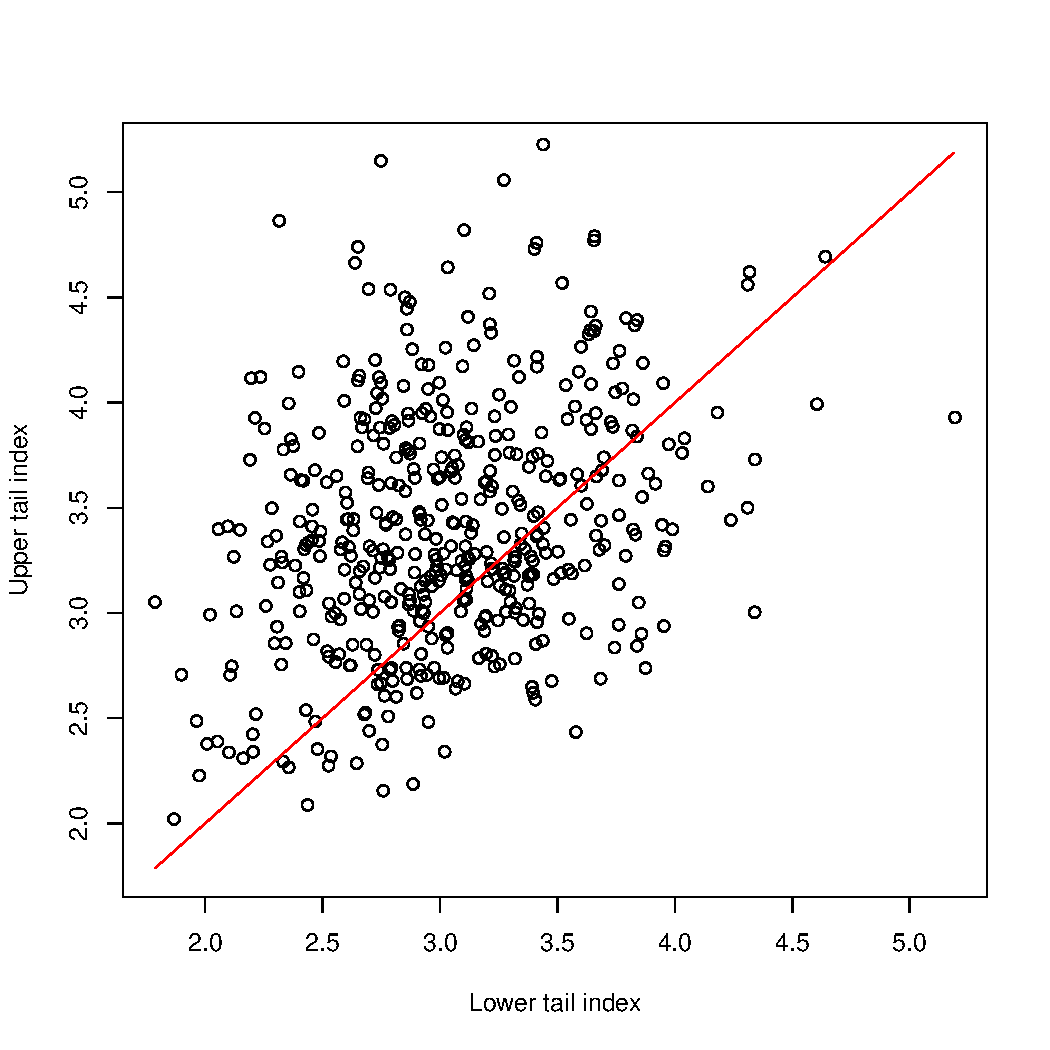
\includegraphics[scale=0.5]{SP500_tail_indices.pdf}
  \caption{Tail indices of stocks included in the S\&P 500 index. The tail
    indices are obtained as their Hill estimators. The red line is the line with equal lower- and upper
    tail indices.}
  \label{fig:SP500_tail_indices}
\end{figure}

\subsection{Overview of light-tailed case}
Yin, Bai and Krishnaiah proved in their 1988 paper
\cite{yin:bai:Krishnaiah:1988} the followng result for a $p \times n$
matrix $\bf W$ with iid entries $w_{ij}$ under the assumption $\E
w_{11} = 0$ and $\E w_{11}^4 < \infty$.
\[
\lim_{n \to \infty} \lambda_{\M}\left({1 \over n}\bf{WW'}\right) = \left(
  1 + \sqrt{p \over n}
\right)^2 \E w_{11}
\]


\subsection{Finite $p$: Anderson}
\subsection{Growing $p$: Johnstone, Tao + Vu}

%------------------------------------------------------------------------
\section{The iid heavy-tailed case}

\subsection{$\alpha \in (0,2)$: Overview of existing results: Davis et al., Soshnikov, Auffiner et al.}
\subsection{$\alpha \in (0,2)$: Our extension of these results; only order statistics of $Z_{it}$'s necessary and no sums (proof by the technical result)}
\subsection{$\alpha \in [2,4)$: Overview of existing results: Davis et al., Soshnikov, Auffiner et al.}
\subsection{$\alpha \in [2,4)$: The problem of centering and restrictions on $p_n$}
\subsection{$\alpha \in [2,10/3)$: Our new result for the UNCENTERED sample covariance matrix; only order statistics of $Z_{it}$'s necessary and no sums (proof by the technical result)}
\subsection{$\alpha \in [10/3,4)$: A conjecture with partial proof for the UNCENTERED sample covariance matrix)}

%------------------------------------------------------------------------
\section{Extension to linear dependence, two-sided filters}

\subsection{$\alpha \in (0,10/3)$: Eigenvalues of the sample covariance matrix}
\subsection{$\alpha \in [10/3,4)$: Eigenvalues of the CENTERED sample covariance matrix}
\subsection{$\alpha \in [2,4)$ and $p/n \to \gamma \in (0,1]$: Eigenvalues of the sample covariance matrix using Auffinger's result}
\subsection{Point process convergence}

%------------------------------------------------------------------------
\section{Applications of the results in the previous section}

\subsection{Ratio of second to largest eigenvalue (to power become uniform), self-normalizing sums, ratio of largest eigenvalue to trace, simulations, figures,...}
\subsection{Functions acting on the eigenvalues}
\subsection{Figures: Ratios of consecutive eigenvalues, illustrations for financial data, ...}
\subsection{S\&P data using ranks}
For real financial data, it is unreasonable to expect all
the time series under consideration to have the same tail index. So a
preocedure of standardization has to be adopted. In this section we
use the rank transform.

Suppose we have $p$ time series each of length $n$ and have arranged
them in a $p\times n$ matrix $X_{it}$, where $i = 1, 2, \dots, p$ and
$t=1,2, \dots, n$. For each row of $X$, we transform it as
\begin{eqnarray*}
  R_{it} &=& -\left[
    \log \left({1 \over n+1} \sum_{\tau=1}^n \1_{X_{i\tau} \leq X_{it}} \right)
  \right]^{-1}
\end{eqnarray*}
When $X_{it}$ are iid for each $i$, the argument to the $\log$
function is asymptotically uniformly distributed as $n \to \infty$,
and hence $R_{it}$ is a standard Fr\'echet r.v.

Figure \ref{fig:EigenRatio} shows the ratio of successive eigenvalues
of the matrix $a_{np}^{-2}RR'$, where the rows of matrix $R$ comprise
the rank-transformed sequences of a number of selected time series
in the S\&P 500 index.
\begin{figure}[htb!]
  \centering
  \subfigure[]{
    \includegraphics[scale=0.40]{EigenRatioSP500_100_shown.pdf}
  }
  \subfigure[]{
    \includegraphics[scale=0.40]{EigenRatioSP500_200_shown.pdf}
  }
  \subfigure[]{
    \includegraphics[scale=0.40]{EigenRatioSP500_300_shown.pdf}
  }
  \subfigure[]{
    \includegraphics[scale=0.40]{EigenRatioSP500_400_shown.pdf}
  }
  \caption{$\lambda_{(i+1)} / \lambda_{(i)}$ versus $i$}
  \label{fig:EigenRatio}
\end{figure}
It is seen that, as $i \to \infty$, $\lambda_{(i+1)} / \lambda_{(i)}
\to 1$. This is in fact expected based on the theory explained in the
previous sections. Suppose the sequences are iid and serial
correlations are absent, i.e. the matrix $M=H H'$ has only one eigen
value. Then it is clear ${\lambda_{(i+1)} \over
  \lambda_i}=\left({\Gamma_i \over
    \Gamma_{i+1}}\right)^{2/\alpha}=\left(1 - {E_{i+1} \over E_1 + E_2
    + \dots E_{i+1}}\right)^{2/\alpha} \to 1$, where $E_k,
k=1,2,\dots,i+1$ are iid. exponential rv.

%------------------------------------------------------------------------
\section{A further extension: The sample autocovariance function}

\subsection{$\alpha \in (0,10/3)$: Eigenvalues of the sample autocovariance matrix}
\subsection{$\alpha \in [10/3,4)$: Eigenvalues of the CENTERED sample autocovariance matrix}

%------------------------------------------------------------------------
\section{Applications of the results for the autocovariance function}

\subsection{Sums of largest eigenvalues vs.~ largest eigenvalues of sums, application to real data + plots}
\subsection{Explanation of these plots in the separable case, discussion of the two methods to ensure real eigenvalues, link to Lam + Yao}

%------------------------------------------------------------------------
\section{Non-linear theory, independent rows + large deviations, SV and GARCH, SV with multivariate Gaussian and t-distributed noise}
%------------------------------------------------------------------------
\section{Future directions, discussion of the conjecture}


%------------------------------------------------------------------------
\appendix 
\section{Regular variation, large deviations and point processes}
\section{The key technical result to identify the largest eigenvalues with the order statistics of the squares of the matrix entries in the iid case}
\section{A lemma which shows that the sample covariance matrix is approximated by its diagonal in the iid case (more involved than simple matrix norms)}
\section{The Proofs}












%-----------------------------------------------------------------------
%Bibliography
%Bibliography
\begin{thebibliography}{99}
\baselineskip12pt
%AAAAAAAAAAAAAAAAAAAAAAAAAAAAAAAAAAAAAAAAAAAAAAAAAAAAAAAAAAAAAAA
\bibitem{anderson:1963}
{\sc Anderson, T.W.,}\ (1963)
{\em Asymptotic theory for principal component analysis.}  {\em Ann.~Math.~Statist.} {\bf 34}, 122--148.
%\bibitem{anderson:guionnet:zeitouni:2008}
%{\sc Anderson, G.W., Guionnet, A. and Zeitouni, O.}\ (2008)
%{\em An Introduction to Random Matrices.}  Cambridge
%University Press, Cambridge (UK).

\bibitem{auffinger:arous:peche:2009}
{\sc Auffinger, A., Ben Arous, G. and P\'ech\'e, S.}\ (2009)
Poisson convergence for the largest eigenvalues of heavy tailed random
matrices.
{\em Ann. Inst. H. Poincar\'e, Probab. Statist.} {\bf 45}, 589--610.
%BBBBBBBBBBBBBBBBBBBBBBBBBBBBBBBBBBBBBBBBBBBBBBBBBBBBBBBBBBBBBBB
%\bibitem{bai:silverstein:2010}
%{\sc Bai, Z. and Silverstein, J.W.}\ (2010)
%{\em Spectral Analysis of Large Dimensional Random Matrices.} 2nd
%Edition. Springer, New York.
%\bibitem{belinschi:dembo:guionnet:2009}
%{\sc Belinschi, S.,  Dembo, A. and Guionnet, A.}\ (2009)
%Spectral measure of heavy tailed band and covariance random matrices.
%{\em Comm. Math. Phys.}  {\bf 289}, 1023--1055.
%\bibitem{arous:guionnet:2008}
%{\sc  Ben Arous, G. and  Guionnet, A.} \ (2008)
%The spectrum of heavy tailed random matrices.  {\em Comm. Math. Phys.}
%{\bf 278}, 715--751.
\bibitem{bhatia:1997}
{\sc Bhatia, R.}\ (1997)
{\em Matrix Analysis.} Springer, New York.
\bibitem{bingham:goldie:teugels:1987}
{\sc Bingham, N.H., Goldie, C.M.\ and Teugels, J.L.}\ (1987)
{\em Regular Variation.} Cambridge University Press, Cambridge.
%\bibitem{bose:hazra:saha:2009}
%{\sc Bose, A., Subhra Hazra, R. and  Saha, K.}\ (2009)
%Limiting spectral distribution of circulant type matrices
%with dependent inputs.  {\em Electron. J. Probab.}  {\bf 14},
%2463--2491.
%\bibitem{bose:hazra:saha:2010}
%{\sc Bose, A., Subhra Hazra, R. and  Saha, K.}\ (2010)
%Spectral norm of circulant type matrices with heavy tailed entries.
%{\em Electron. Commun. Probab.}  {\bf 15}, 299--313.
%CCCCCCCCCCCCCCCCCCCCCCCCCCCCCCCCCCCCCCCCCCCCCCCCCCCCCCCCCCCCCCC
\bibitem{cline:hsing:1998}
{\sc Cline, D.B.H. and Hsing, T.}\ (1998)
Large deviation probabilities for sums of random variables
with heavy or subexponential tails. Technical report.
Statistics Dept., Texas A\&M University. %Available as \begin{verbatim}http://www.stat.tamu.edu/~dcline/Papers/large5.pdf \end{verbatim}
%DDDDDDDDDDDDDDDDDDDDDDDDDDDDDDDDDDDDDDDDDDDDDDDDDDDDDDDDDDDDDDD
\bibitem{davis:resnick:1985}
{\sc
Davis, R.A. and Resnick, S.I.}\ (1985)
Limit theory for moving averages of random variables
with regularly varying tail probabilities.
{\em Ann. Probab.} {\bf 13}, 179--195.
\bibitem{davis:pfaffel:stelzer:2014}
{\sc Davis, R.A., Pfaffel, O. and Stelzer, R.}\ (2014)
Limit theory for the largest eigenvalues of
sample covariance matrices with heavy tails.
{\em Stoch. Proc. Appl.} {\bf 124}, 18--50.

\bibitem{denisov:dieker:shneer:2008}
{\sc Denisov, D., Dieker, A.B. and Shneer, V.}\ (2008)
Large deviations for random walks under subexponentiality:
the big-jump domain.
{\em Ann. Probab.} {\bf 36}, 1946--1991.

%EEEEEEEEEEEEEEEEEEEEEEEEEEEEEEEEEEEEEEEEEEEEEEEEEEEEEEEEEEEEEEE

\bibitem{embrechts:goldie:1980}
{\sc Embrechts, P. and Goldie,C.}\ (1980)
On closure and factorization theorems for subexponential and related
distributions. {\em J. Austral. Math. Soc.,} Ser. A {\bf 29}, 243--256.

%\bibitem{embrechts:kluppelberg:mikosch:1997}
%{\sc Embrechts, P., Kl\"uppelberg, C. and Mikosch, T.}\ (1997)
%{\em Modelling Extremal Events for Insurance and Finance.}
%Springer,  Berlin.

%GGGGGGGGGGGGGGGGGGGGGGGGGGGGGGGGGGGGGGGGGGGGGGGGGGGGGGGGGGGGGGG

\bibitem{gohberg:goldberg:krupnik:2000}
{\sc Gohberg, I., Goldberg, S. and N. Krupnik}\ (2000)
{\em Traces and Determinants of Linear Operators.} Birkh\"auser, Basel.

\bibitem{johnstone:2001}
{\sc Johnstone, I.M.}\ (2001)
{\em on the distribution of the largest eigenvalue in principal component analysis.} {\em Ann.~Statist.} {\bf 29} (2), 295--327.

%MMMMMMMMMMMMMMMMMMMMMMMMMMMMMMMMMMMMMMMMMMMMMMMMMMMMMMMMMMMMMMM

\bibitem{mikosch:samorodnitsky:2000}
{\sc Mikosch, T. and Samorodnitsky, G.} \ (2000)
The supremum of a negative drift random walk with
dependent heavy-tailed steps. {\em Ann. Appl. Probab.} {\bf 10}, 1025--1064.

%NNNNNNNNNNNNNNNNNNNNNNNNNNNNNNNNNNNNNNNNNNNNNNNNNNNNNNNNNNNNNNN

\bibitem{nagaev:1979}
{\sc Nagaev, S.V.}\ (1979)
Large deviations of sums of independent random
variables.
{\em Ann. Probab.} {\bf 7}, 745--789.

%PPPPPPPPPPPPPPPPPPPPPPPPPPPPPPPPPPPPPPPPPPPPPPPPPPPPPPPPPPPPPPP

\bibitem{petrov:1995}
{\sc Petrov, V.V.} (1995)
{\em Limit Theorems of Probability Theory.} Oxford University Press,
Oxford.

%RRRRRRRRRRRRRRRRRRRRRRRRRRRRRRRRRRRRRRRRRRRRRRRRRRRRRRRRRRRRRRR

\bibitem{resnick:1987}
{\sc Resnick, S.I.}\ (1987)
{\em Extreme Values, Regular Variation, and Point Processes.}
Sprin\-ger, New York.

\bibitem{resnick:2007}
{\sc Resnick, S.I.}\ (2007)
{\em Heavy-Tail Phenomena: Probabilistic and Statistical Modeling.}
Springer, New York.

%SSSSSSSSSSSSSSSSSSSSSSSSSSSSSSSSSSSSSSSSSSSSSSSSSSSSSSSSSSSSSSS

\bibitem{samorodnitsky:taqqu:1994}
{\sc Samorodnitsky, G. and Taqqu, M.S.}\ (1994)
{\em Stable Non-Gaussian Random Processes.
Stochastic Models with Infinite Variance.} Chapman and Hall, London.

%\bibitem{soshnikov:2004}
%{\sc Soshnikov, A.}\ (2004)
%Poisson statistics for the largest eigenvalues of Wigner matrices with
%heavy tails. {\em Electr. Comm. Probab.} {\bf 9}, 82--91.

\bibitem{soshnikov:2006}
{\sc Soshnikov, A.}\ (2006)
Poisson statistics for the largest eigenvalues in random matrix
ensembles.
In: {\em Mathematical Physics of Quantum Mechanics.} Lecture Notes in
Physics {\bf 690}. Springer, Berlin, pp. 351--364.

\bibitem{tao:vu:2012}
{\sc Tao, T. and Vu, V.}\ (2012)
Random covariance matrices; universality of local statistics of eigenvalues.
{\em Ann.~Probab.} {\bf 40} (3), 1285--1315.

\bibitem{yin:bai:Krishnaiah:1988}
{\sc Y.Q. Yin and Z.D. Bai and P.R. Krishnaiah}\ (1988)
On the Limit of the Largest Eigenvalue of the Large Dimensional Sample
Covariance Matrix.
{\em Probability Theory and Related Fields} {\bf 78}, 509--521.

\end{thebibliography}
\end{document}